% !TEX root = ../thesis.tex
% !TeX spellcheck = en_US

\section{Overview and Context}

	% Used by agents for wayfinding
	The primary goal of the hybrid routing algorithm is to provide a more accurate path planning for agent based simulations than normal graph based routing, which is integrated into the MARS framework.
	Such major goal implies several constrains on the architecture and design of the software.
	
	\subsection{Requirements}
	
		Functional requirements of the resulting software can be formulated quite easily, since this is not a large commercial product.
		The hybrid routing algorithm should determine an optimal path between two locations following ways and traversing open spaces based on a configurable weight function.
		Therefore, the geospatial data basis may contain a road network data and obstacles, which are features that should be avoided on paths through open spaces.
		
		More complex and time consuming are the quality requirements.
		Because this is not part of a commercial software development, these requirements were not officially and formulated.
		Nonetheless, they exist and consist of the following aspects.
	
		The largest quality requirement in terms of effort is performance.
		It affects large parts of the software architecture since the resulting algorithm, dispite its complexity, should ideally have a negligible impact on the overall performance of a simulation.
		Routing algorithms and engines often consist of two steps, a preprocessing and query answering step.
		In order to create fluent and fast simulations, the performance of answering numerous routing requests must be as good as possible.
		The time needed for preprocessing is of less relevance.
		
		A rather obvious requirement is the correctness of resulting routes.
		The answer of a routing query must return the shortest route according to a given weight function for the underlying edges.
		Even when using an approximation algorithm to determine shortest paths, the results can be checked against all other possible paths to verify the optimality of the resulting path.
		
		Another quality requirement is the closeness of the resulting routes to real pedestrian behavior.
		Unfortunately, this can hardly be measured without having extensive data of real world pedestrians in real world locations.
		However, the overall trajectory of a calculated route should ideally be identical to a real world pedestrian trajectory and should at least make sense to an observer without additional knowledge of the real world location.
		Furthermore, real pedestrian behavior is not part of the shortest path calculations but is instead a task for realistic agent modeling.

		Next to the software specific requirement, the overall code itself should of course be well documented and tested.
	
	\subsection{Constrains}
	\label{subsec:constrains}
		
		% Well integrated into MARS and NTS, no new dependencies
		One major constraint is the integration of the hybrid routing algorithm into the \term*{MARS} framework to make the use as easy as possible and to centralize the code base for better maintenance.
		This means the programming language will be C\# and because MARS uses the \term{NetTopologySuite} (\term*{NTS}) as basis for all major geospatial operations, this algorithm will be based on this library as well.
		
		The planned integration into another code base affects the management of dependencies.
		On the one hand, the amount dependencies which are not already part of the target code base should be kept to a minimum.
		On the other hand, using only libraries, on which the target code base depends as well, is not always possible due to version mismatches.
		However, the latter case can be avoided or treated in a way that the mismatch disappears or doesn't lead to compatibility problems.
	
	% Diagram with MARS Agent using my hybrid algorithm
	
\section{Components}
\label{sec:components}

	% Generator classes, HybridVisibilityGrahp class and helper functions
	Since this works resides in a rather technical and algorithmic oriented area, there are not many components needed to implement a hybrid routing approach.
	The two most important parts are the graph generation and handling of routing requests.
	
	Because routing requests should be handled entirely within the resulting graph, meaning without the need of additional generators, some of the generator tasks are within the graph component.
	
	Using the implementation therefore has two entry points:
	The generator, which initially creates the routing graph, and the graph itself to which routing requests can be made.
	Due to the chosen construction and handling of arbitrary locations, the graph itself might generate new nodes and edges.
	This is needed to connect the arbitrarily chooseable source and target locations, which is describes in \cref{sec:answering-queries} with more details.
	
	\begin{figure}[h]
		\begin{figcenter}
			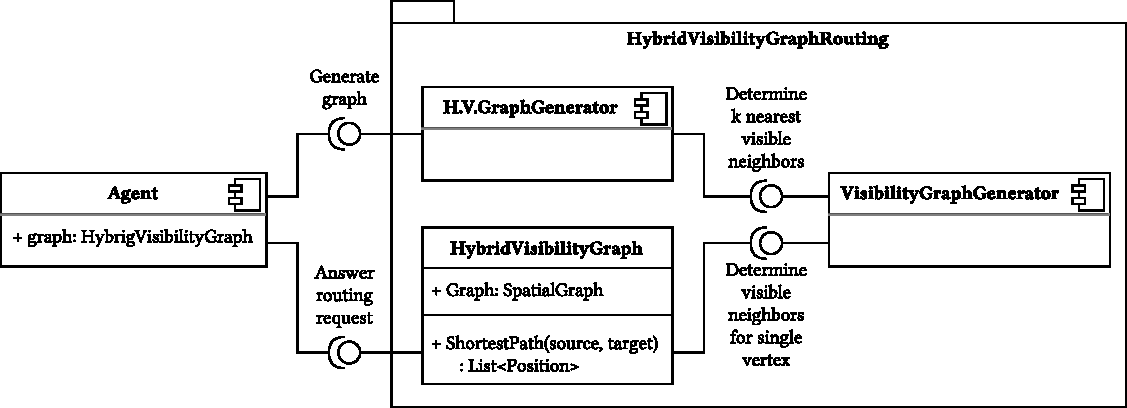
\includegraphics[width=\textwidth]{images/components.pdf}
		\end{figcenter}
		\caption{The relevant components of the resulting implementation.}
	\end{figure}

\section{Deployment view}

	% published in MARS

\section{Combination of routing algorithms}
\label{sec:combining-routing-algorithms}

	This section describes the core aspect of this thesis:
	The decision of a strategy to combine graph and geometric based routing algorithms.
	
	In the following subsections, four approaches are discussed of which the last one seemed to be the most promising.
	The first three are using any normal graph based routing algorithm, like A* or Dijkstra, in combination with the geometric continuous Dijkstra paradigm.
	Only the last and further pursued approach uses visibility graphs for routing.
	
	% Ad-hoc creation of edges by stopping A* and continuing with wavefront algorithm
	\subsection{Ad hoc generation of edges}
	
		The idea of an ad hoc generation of edges is the following:
		Whenever the graph routing algorithm reaches a crossing of ways, it's paused and the continuous Dijkstra algorithm is started.
		Since no target vertex is defined, the geometric routing will be stopped after the furthest wavelet reached a certain distance.
		The continuous Dijkstra approach actually creates a shortest path map, so the shortest paths of all reached vertices are calculated yielding a series of edges.
		These edges are then added to the graph for the paused graph based routing algorithm.
		
		In a real world example for this approach would be a pedestrian walking down a road but then crossing a park for a shortcut before continuing to follow the roads again.
		Doing the shortcut was not planned but an ad hoc decision just as the algorithm would do.
		
		The advantage of this approach is the realistic behavior of pedestrians not planning the route in beforehand.
		In fact Teknomo and Millonig introduced a routing mechanism for agent based simulations with the assumption of little to no apriori knowledge of agents about their environment \cite{teknomo-millonig-routing}.
		
		One disadvantage is a relatively high complexity since no standard algorithm from frequently used software frameworks support a pause functionality, so any routing algorithm has to be manually adjusted or implemented from scratch.
		
		Also this approach will likely cause performance issues.
		When using Dijkstra as graph based routing algorithm, $\bigo{|V|}$ many vertices are visited, which leads to $\bigo{|V|}$ routing requests using the geometric continuous Dijkstra algorithm.
		Because a simple caching of the shortest path map is not possible, at least not without a smart and complex caching strategy, this decreases the runtime of the whole routing process significantly.
		Even when using the continuous Dijkstra approach from Hershberger and Suri \cite{hershberger-suri} with only $\bigo{n \log n}$ time requirement, the number $n$ of vertices in obstacles is expected to be much higher than the size of $V$.
		
		Another aspect against this approach is the hypothesis that an ad hoc generation of edges will probably not change the resulting shortest path compared to a precomputed graph consisting of all possible edges.
		An argumentation for the correctness of this hypothesis can be sketched as follows.
		
		Assume that the ad hoc generation starts at each road junction vertex $j$ and stops when a certain condition is fulfilled (for example only generating paths of a certain length).
		When the graph routing algorithm reaches an unvisited junction vertex $j$ from some other vertex $v$, it either used a road edge or preprocessed edge to get there. Therefore, the following two cases exist:
		\begin{itemize}
			\item In case a preprocessed edge was used, then the shortest path from $v$ to $j$ would be identical when using a completely preprocessed graph containing this exact edge $(v, j)$.
			\item In case a road edge was used to get to $j$, then there are two sub-cases.
			\begin{itemize}
				\item In case the road edge was in deed the optimal path to $j$, it would have been used in a preprocessed graph as well.
				\item In case the road edge was not the optimal path, then the ad hoc generation stopped before reaching $j$ (due to the distance or any other stopping condition) and the edge $(v, j)$ was never added.
			\end{itemize}
		\end{itemize}
		Even though, this is not a formal proof, generating a preprocessed graph and using a normal routing algorithm is probably as least as good as using the ad hoc generation approach.
	
	% Concurrent routing: Use A* and wavefront in parallel and merge the results
	\subsection{Concurrent routing}
	
		A different approach would be two concurrent routing queries, one on the normal road graph and one using a visibility graph or a similar generated graph.
		Having the two shortest paths, one could merge them into one path, which would consist of alternating segments from the one or the other graph.
		To merge them, first determine the intersection points and for each pair of segments, choose the better one based on a weight function.
		
		The most prominent advantage is the simplicity of the routing requests, since known routing algorithms could be used.
		Therefore, it would be rather simple to implement and speed up techniques could be used.
		
		However, there is a major disadvantage, which is the uncertainty, that the two paths are actually intersecting at any point.
		Even if they are intersecting, a single intersection on a long route is not very helpful.
		Only if the two routes are intersecting frequently enough, this approach could actually result in good routes.
	
	% Concurrent routing for segments (e.g. start new routing calls every 100m)
	\subsection{Concurrent routing on smaller segments}
	
		This approach is very similar to the one above, however, it tries to fix the uncertainty of intersections between the two resulting paths.
		There are multiple ways to ensure that there are enough intersections or to otherwise guarantee small enough segments to merge.
		
		One way is to stop the routing after a certain distance stopping at the next available vertex.
		After stopping for the first time, there are two such vertices, one where the graph based routing stopped and one where the routing on the generated graph stopped.
		From each vertex, two new routing queries start and stop after a certain distance.
		This is continued until one query reaches the target.
		On the one hand, this would guarantee small enough segments for later merging, on the other hand, this results in $\bigo{2^n}$ many routing queries.
		Even though each query is short, this approach would probably not scale very well.
		
		A different approach for smaller segments would be to first get the shortest path on the road graph.
		Having this path, it is split up into $n$ segments of certain length.
		From the end vertex of each segment $s_i$, a shortest path query to the start of all other segments $s_{i+1}, s_{i+2}, ..., s_n$ is performed including one query from the end of $s_i$ to the target vertex.
		Unfortunately this results in $O(n^2)$ more routing queries.
		Finally, all these queries on the generated graph can be merged together with the query result of the road graph to form a new intermediate graph.
		Finally, one last routing query on this intermediate graph is performed to get the final optimal routing result.
		
		There are probably more possible ways to ensure a sufficient amount of segments or intersection, however, this idea was not further continued.
		
		Unfortunately, both approaches have a worse time complexity than any popular routing algorithms including pure geometric routing.
		Even though the second idea might work well for appropriate segments lengths, the complexity and definite time overhead make it an unfavorable choice.
	
	% Merge of networks
	\subsection{Merge an existing network with a visibility graph}
	
		The last approach, which is the currently used one, generates a visibility graph and merges it with the existing road graph.
		The actual merge operation is very simple:
		Whenever a road edge and a visibility edge intersect, split the edges, create a new vertex there and connect the split edges accordingly.
		
		Even though, this approach is simple and still fast, there is the disadvantage of the graph size.
		A visibility graph is large and in most cases it will contain many more edges than the road graph, which negatively affects the routing performance.
		
		Another disadvantage is the time complexity of the merge operation.
		All edges have to be considered and most edges will even be considered multiple times, depending on the number of intersections.
		This leads to a time complexity of $\Omega(|E_R| + |E_V|)$ for the routing graph edges $E_R$ and visibility edges $E_V$.
		However, a complete graph has the highest number of edge crossings, which gives the upper bound of $\bigo{|E|^2}$ for the merge operation.
		Fortunately, road networks are very sparse and often have a node degree between three and six \cite{zhao-analysis-osm-bejing}\cite{boeing-osmnx}, resulting in a much better runtime behavior.
		\todo[inline]{Maybe analyze this myself for e.g. Germany?}
		\todo[inline]{Link to possible optimizations discussed in later chapters}
		
		However, the advantages are more important.
		As already mentioned, this strategy is simple and fast, compared to the time complexities above, only makes one routing query and enabled the use of speed up methods.
